\documentclass{article}

\usepackage[utf8]{inputenc}
\usepackage{microtype}
\usepackage{geometry}

\usepackage{amsmath}
\usepackage{graphics}
\usepackage{tikz}

% Tweak spacing of descriptions.
\usepackage{enumitem}
\setlist[description]{topsep=1ex, labelsep=0.6ex}

% Tweak captions.
\usepackage[font=sf,
            labelfont=bf,
            labelsep=period,
            singlelinecheck=off]{caption}

% Make float text and math sans serif.
\usepackage[font=sf]{floatrow}
\usepackage{sansmath}
\usepackage{etoolbox}
\AtBeginEnvironment{table}{\sansmath}
\AtBeginEnvironment{figure}{\sansmath}
\floatsetup[table]{capposition=top,  % Table captions on top.
                   justification=justified}  % Don't center by default.

% Nice formatting for \textwidth tables.
\usepackage{tabularx}

\usepackage[noblocks]{authblk}
\renewcommand{\Affilfont}{\small}

\usepackage[pdfborder={0 0 0}]{hyperref}

% \usepackage[style=nature]{biblatex}
% \addbibresource{supporting_information.bib}
\usepackage[numbers, round, comma, sort&compress]{natbib}
\usepackage{hypernat}
% PNAS style: no brackets in reference list.
\makeatletter 
\renewcommand\@biblabel[1]{#1.} 
\makeatother

% PNAS style: square brackets around equation labels and all in
% boldface, boldface equation number in references.
\usepackage{mathtools}
\newtagform{brackets}{\bf[}{]}
\usetagform{brackets}
\renewcommand{\eqref}[1]{\textbf{\ref{#1}}}

\renewcommand{\thesection}{S\arabic{section}}
\renewcommand{\thefigure}{S\arabic{figure}}
\renewcommand{\thetable}{S\arabic{table}}
\newcommand{\sectionname}{Section}
\renewcommand{\sectionautorefname}{\sectionname}
\renewcommand{\figurename}{Fig.}
\renewcommand{\figureautorefname}{\figurename}

\usepackage{xr}
\externaldocument{extended_data_fig_1}

\newcommand{\md}{\mathrm{d}}
\DeclareMathOperator{\Uniform}{Uniform}
\DeclareMathOperator{\Triangular}{Triangular}
\DeclareMathOperator{\Lognormal}{Lognormal}
\DeclareMathOperator{\BetaPERT}{Beta-PERT}

\title{Supporting Information for\\
  \emph{Effectiveness of UNAIDS targets and HIV vaccination across 127
    countries}}

\author[a,1]{Jan Medlock}
\affil[a]{Department of Biomedical Sciences,
  Oregon State University,
  106 Dryden Hall,
  Corvallis, OR 97331-4801,
  USA}
\author[b]{Abhishek Pandey}
\author[b]{Alyssa S.~Parpia}
\author[b]{Amber Tang}
\author[b]{Laura A.~Skrip}
\author[b]{Alison P.~Galvani}
\affil[b]{Center for Infectious Disease Modeling and Analysis,
  Yale School of Public Health,
  135 College Street,
  New Haven, CT 06510-2483,
  USA}
\affil[1]{To whom correspondence should be addressed.
  Email: \href{mailto:jan.medlock@oregonstate.edu}
  {\texttt{jan.medlock@oregonstate.edu}}.}


\begin{document}

\maketitle

We developed a mathematical model of HIV transmission and progression
that stratifies HIV infection into acute, chronic undiagnosed, chronic
diagnosed, chronic treated, chronic virally suppressed, and AIDS,
along with uninfected unvaccinated and vaccinated people
(\autoref{model} \& \autoref{model_diag}), tailored to
each of 127 countries.  Simulations of our model project the number of
people in each HIV stratum from 2015 to 2035, from which statistics
such as prevalence and incidence were calculated.  To evaluate the
impact of the 90--90--90 and 95--95--95 UNAIDS goals, model transition
rates were adjusted dynamically to meet intervention goals for
diagnosis, treatment, viral suppression, and vaccination coverage
(\autoref{targets}).  Data and estimates from many sources, including
The World Bank and UNAIDS, were used to parametrize the model
(\autoref{data_sources}).  Country-specific transmission rates were
fitted to estimates of the historical trajectories of incidence and
prevalence, spanning from as early as 1990 for some countries
(\autoref{model_fitting}). For every scenario of intervention
combinations, we conducted 1000 model simulations, sampling values of
model parameters from empirical distributions for each simulation, and
reported the results with median and percentiles
(\autoref{uncertainty}).

\begin{figure}
  \centering
  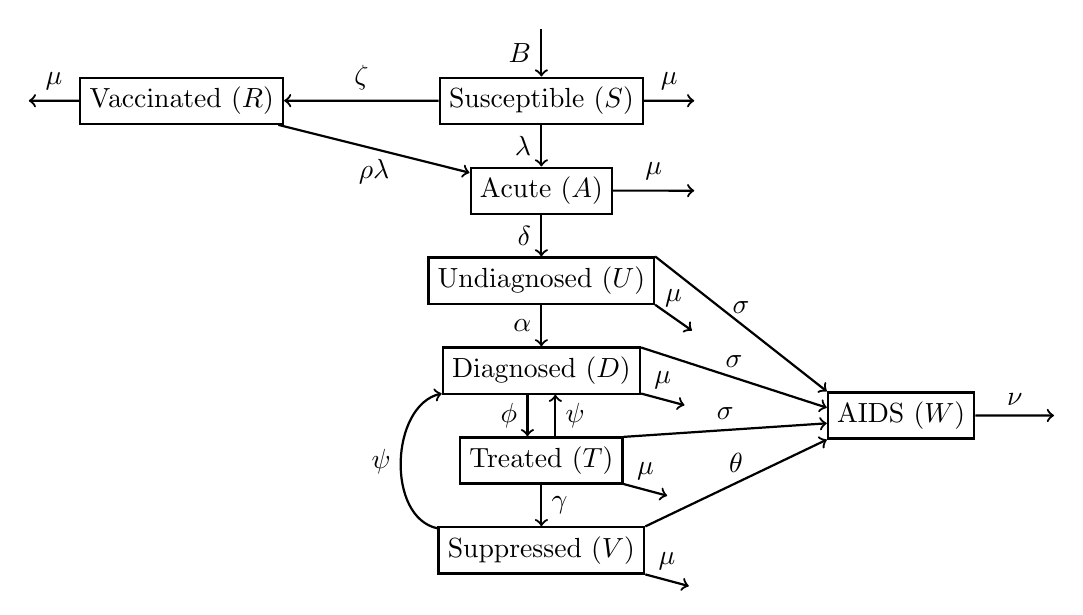
\begin{tikzpicture}[
  thick,
  scale = 1.142,
  compartment/.style = {draw},
  ]

  \node at (0, 5)
  [compartment, name = Susceptible] {Susceptible ($S$)};

  \node at (-4, 5)
  [compartment, name = Vaccinated] {Vaccinated ($R$)};

  \node at (0, 4)
  [compartment, name = Acute] {Acute ($A$)};

  \node at (0, 3)
  [compartment, name = Undiagnosed] {Undiagnosed ($U$)};

  \node at (0, 2)
  [compartment, name = Diagnosed] {Diagnosed ($D$)};

  \node at (0, 1)
  [compartment, name = Treated] {Treated ($T$)};

  \node at (0, 0)
  [compartment, name = Suppressed] {Suppressed ($V$)};

  \node at (4, 1.5)
  [compartment, name = AIDS] {AIDS ($W$)};

  \draw [->] (Susceptible) to node [left] {$\lambda$} (Acute);

  \draw [->] (Susceptible) to node [above] {$\zeta$} (Vaccinated);

  \draw [->] (Vaccinated) to node [below] {$\rho \lambda$} (Acute);

  \draw [->] (Acute) to node [left] {$\delta$} (Undiagnosed);

  \draw [->] (Undiagnosed) to node [left] {$\alpha$} (Diagnosed);

  \draw [->] (Diagnosed.240) to node [left] {$\phi$} (Treated.120);

  \draw [->] (Treated.60) to node [right] {$\psi$} (Diagnosed.300);

  \draw [->] (Treated) to node [right] {$\gamma$} (Suppressed);

  \draw [->] (Suppressed) to [out = 168, in = 193] node [left] {$\psi$} (Diagnosed);

  \draw [->] (Undiagnosed.12) to node [above] {$\sigma$} (AIDS.162);

  \draw [->] (Diagnosed.13) to node [above] {$\sigma$} (AIDS.174);

  \draw [->] (Treated.16) to node [above] {$\sigma$} (AIDS.186);

  \draw [->] (Suppressed.13) to node [above] {$\theta$} (AIDS.198);

  \draw [<-] (Susceptible) to node [left] {$B$} +(90: 0.8);

  \draw [->] (Susceptible) to node [above] {$\mu$} +(0: 1.7);

  \draw [->] (Vaccinated) to node [above] {$\mu$} +(0: -1.7);

  \draw [->] (Acute) to node [above] {$\mu$} +(0: 1.7);

  \draw [->] (Undiagnosed.348) to node [above] {$\mu$} +(325: 0.5);

  \draw [->] (Diagnosed.347) to node [above] {$\mu$} +(345: 0.5);

  \draw [->] (Treated.344) to node [above] {$\mu$} +(345: 0.5);

  \draw [->] (Suppressed.347) to node [above] {$\mu$} +(345: 0.5);

  \draw [->] (AIDS) to node [above] {$\nu$} +(0: 1.7);

\end{tikzpicture}


%%% Local Variables:
%%% mode: latex
%%% TeX-master: "model"
%%% End:

  \caption{Model diagram.}
  \label{model_diag}
\end{figure}

The model simulation and analysis tools, written in Python, are
publicly available \cite{medlock2016-git}.


\section{Model structure}
\label{model}

Within each country, our model divides people aged $15$\;years and
older into non-overlapping HIV states.  We focused on this age group
because it accounts for the vast majority of global PLHIV
\cite{UNICEF}, 93\% in 2014; because population-level HIV estimates
and demographic data are typically only estimated for ages $15$--$49$;
and to capture the continuing burden of infections in people ages $50$
and older.  Our model has 8 HIV states (\autoref{model_diag}):
susceptible to HIV infection ($S$ is the number of people
susceptible), vaccinated against HIV ($R$), acute HIV infection ($A$),
undiagnosed HIV infection ($U$), diagnosed but untreated HIV infection
($D$), treated without viral suppression ($T$), viral suppression
($V$), and having AIDS ($W$).

Transitions between model states are governed by a system of
differential equations parametrized using values found in other
studies, along with transmission rates derived from UNAIDS estimates
of incidence and prevalence (\autoref{model_param}).  The model is
deterministic, but uncertainty in the parameters was treated by
running the model 1000 times with samples from the parameter
distributions (\autoref{uncertainty}) and summarizing the model
outcomes using the median and percentiles.  Each country was modeled
separately (Extended Data
Figs.~\ref*{effectiveness_Afghanistan}--\ref*{effectiveness_Zimbabwe})
and the country simulations were aggregated to calculate global and
regional outcomes (Extended Data
Figs.~\ref*{effectiveness_Global}--\ref*{effectiveness_Western_Europe}).

\begin{table}
  \caption{Model parameters.}
  \label{model_param}
  \begin{tabularx}{\textwidth}{lXlll}
    \hline
    & Definition & Value & References
    \\ \hline
    $\mu$ & Background death rate
    & Country specific, Data Set 2
    & \cite{World_Development_Indicators2013-ee}
    \\
    $\kappa$ & Recruitment rate
    & Country specific, Data Set 2
    & \cite{World_Development_Indicators2013-ee, WorldBankpg}
    \\
    $\delta$ & Rate of progression from acute infection
    & $\Triangular(2, 4.14, 9.6)\;\text{y$^{-1}$}$
    & \cite{Hollingsworth2008-iy}
    \\
    $\sigma$ & Rate of developing AIDS without viral suppression
    & $0.1064\;\text{y$^{-1}$}$ & \cite{Morgan2002-cq}
    \\
    $\theta$ & Rate of developing AIDS with viral suppression
    & Eq.~\eqref{theta} & ---
    \\
    $\gamma$ & Rate of viral suppression
    & $\Uniform(0.5, 1.5)\;\text{y$^{-1}$}$
    & \cite{Currie2009-yz}
    \\
    $\nu$ & Death rate from AIDS & $0.5\;\text{y$^{-1}$}$
    & \cite{Morgan2002-cq}
    \\
    $\rho$ & Vaccine efficacy & 50\%\,[30\%, 70\%] & ---
    \\
    $\omega$ & Reduction in life expectancy with viral suppression
    & $\Uniform(5, 8)\;\text{y}$
    & \cite{Samji2013-kf, Unaids2014-ue}
    \\
    $\tau_{A}$ & Transmissibility per coital act during acute phase
    & $\Triangular(0.0039, 0.0082, 0.0150)$
    & \cite{Wawer2005-us, Skarbinski2015-ni}
    \\
    $\tau_{U}$ & Transmissibility per coital act after acute phase
    & $\Triangular(0.00077, 0.0014, 0.00251)$
    & \cite{Hughes2012-so}
    \\
    $\epsilon$ & Relative transmissibility per coital act with
    viral suppression & $\BetaPERT(0.08, 0.002, 0.57)$
    & \cite{Donnell2010-xo, attia_2009, wilson_2012, jia_2013,
      rodger_2016}
    \\
    $n$ & Coital acts per year & $\Uniform(96, 108)$
    & \cite{Wawer2005-us, Abdool_Karim2010-cm}
    \\
    $\alpha$ & Diagnosis rate & Eq.~\eqref{diagnosis_rate} & ---
    \\
    $\phi$ & Treatment rate & Eq.~\eqref{treatment_rate} & ---
    \\
    $\psi$ & Rate of relapse to untreated & Eq.~\eqref{relapse_rate} & ---
    \\
    $\zeta$ & Vaccination rate & Eq.~\eqref{vaccination_rate} & ---
    \\ \hline
  \end{tabularx}
  \\[5pt]
  $\Triangular$, $\Uniform$, and $\BetaPERT$ are sampling
  distributions (\autoref{uncertainty}).
  \\
  For vaccine efficacy, $50\%$ was the baseline, and $30\%$ and $70\%$
  were also assessed in sensitivity analysis.
\end{table}

People susceptible to HIV ($S$) are at risk of becoming infected
according to the force of infection ($\lambda$), which depends on the
HIV transmission rate, estimated from the country-specific incidence
and prevalence data (\autoref{model_fitting}), adjusted for the
current number of acutely infected, untreated or ineffectively
treated, and virally suppressed PLHIV.  Upon infection, people
transition into acute infection ($A$), characterized by high viral
loads for an average of 2.90 [95\% confidence interval 1.23,
6.00]\;months \cite{Hollingsworth2008-iy}.  (We converted these
durations to rates like $1 / 2.90\;\text{month$^{-1}$} \approx
4.14\;\text{y$^{-1}$}$ and set the parameter using random samples from
$\Triangular(2, 4.14, 9.6)\;\text{y$^{-1}$}$ to capture the
uncertainty in its value.  See \autoref{uncertainty} for the
definition of $\Triangular(a, b, c)$ and other distributions.)  Acute
infection progresses into the chronic undiagnosed class ($U$), from
which diagnosis occurs at the rate $\alpha$, which is determined by
the country's current diagnosis level and its diagnosis target under
the different scenarios (\autoref{targets}).  Upon diagnosis, people
transition into the diagnosed class ($D$).  From the diagnosed class,
people transition to the treated compartment ($T$) upon starting ART
at the rate $\phi$, dependent on the country's current treatment level
and its treatment target (\autoref{targets}).  Treated people
transition to the viral suppression ($V$) at the rate $\gamma$,
sampled from $\Uniform(0.5, 1.5)\;\text{y$^{-1}$}$: thus, viral
suppression occurs after between 8 months and 2 years on
treatment \cite{Currie2009-yz}.  Disengagement from treatment moves
people from treated ($T$) and viral suppression ($V$) back to the
diagnosed class ($D$) at the rate $\psi$, dependent on the current
level of viral suppression and the country's target
(\autoref{targets}).

PLHIV without viral suppression (compartments $U$, $D$, and $T$)
develop AIDS (compartment $W$) after an average duration of 10.4
years \cite{Morgan2002-cq}, i.e.~with transition rate
$\sigma = 0.1064\;\text{y$^{-1}$}$.  Viral suppression greatly reduces
the rate of progression to AIDS ($\theta$) and improves longevity,
such that life expectancy is only $5$--$8$\;y shorter than average
country-specific life expectancy \cite{Samji2013-kf, Unaids2014-ue}.
This reduction in life expectancy was quantified by randomly sampling
the parameter $\omega$ from $\Uniform(5, 8)\;\text{y}$. Thus, in the
absence of relapse to untreated, the duration of viral suppression is
\begin{equation}
  \frac{1}{\theta + \mu} = \frac{1}{\mu} - \omega - \frac{1}{\nu}.
\end{equation}
The left-hand side of the equation is the time until leaving viral
suppression by either progression to AIDS (at rate $\theta$) or
background mortality (at rate $\mu$).  The right-hand side of the
equation is the life expectancy of uninfected people, minus the
reduction in life expectancy attributable to virally suppressed HIV
infection, minus the duration of the AIDS stage.  Solving for $\theta$
gives the rate of progression to AIDS from viral suppression,
\begin{equation}
  \label{theta}
  \theta = \frac{1}{1/\mu - \omega - 1/\nu} - \mu.
\end{equation}

In the vaccination scenarios, susceptible people are vaccinated at
rate $\zeta$, depending on the country's current vaccination coverage
and its coverage target (\autoref{targets}), transitioning into the
vaccinated compartment ($R$).  The force of infection for vaccinated
people is reduced by the efficacy factor $\rho$.  We took the
base-case efficacy to be $50\%$, but varied it to $30\%$ and $70\%$ in
sensitivity analysis (\autoref{uncertainty}).  We did not model
specific vaccine dose regime, such that implicit in our efficacy
parameter is the assumption that boosters will be used to maintain
efficacy over time.  Without vaccine, $\zeta = 0$.

The background mortality rate ($\mu$) in each of the 127 countries was
collected from published
estimates \cite{World_Development_Indicators2013-ee}.  The recruitment
rate ($\kappa$) into the age $15\;\text{y}$ and older group was set by
the difference between the country's population growth
rate \cite{WorldBankpg} and its background mortality
rate \cite{World_Development_Indicators2013-ee}, as would be true if
the population was at its stable age structure.  (More on these data
sources is in \autoref{data_sources}.)

We also added differential equations to track the cumulative number of
new infections ($Y$) and AIDS deaths ($Z$) over the simulation period.

The model equations are
\begin{equation}
  \label{model_eqns}
  \begin{split}
    \frac{\md S}{\md t} &= \kappa N - \lambda S - \zeta S- \mu S,
    \\
    \frac{\md R}{\md t} & = \zeta S - (1 - \rho) \lambda R - \mu R,
    \\
    \frac{\md A}{\md t} &= \lambda S + (1 - \rho) \lambda R - \delta A - \mu A,
    \\
    \frac{\md U}{\md t} &= \delta A - \alpha U - \mu U - \sigma U,
    \\
    \frac{\md D}{\md t} &=  \alpha U + \psi T + \psi V
    - \phi D - \mu D - \sigma D,
    \\
    \frac{\md T}{\md t} &= \phi D - \psi T - \gamma T - \mu T
    - \sigma T,
    \\
    \frac{\md V}{\md t} &= \gamma T - \psi V - \mu V - \theta V,
    \\
    \frac{\md W}{\md t} &= \sigma U + \sigma D + \sigma T + \theta V -
    \nu W,
    \\
    \frac{\md Y}{\md t} &= \lambda \big[S + (1 - \rho) R\big],
    \\
    \frac{\md Z}{\md t} &= \nu W,
  \end{split}
\end{equation}
with force of infection
\begin{equation}
  \label{force_of_infection}
  \lambda =
  \frac{\xi \big[\beta_A A + \beta_U (U + D + T) + \beta_V V\big]}{N},
\end{equation}
and sexually active population size $N = S + R + A + U + D + T + V$.
We assumed that people with AIDS ($W$) are too sick to be sexually
active.

The relative transmission rates (per unit time), $\beta$, from acute
($A$), unsuppressed ($U$ and $T$), and suppressed infected ($V$)
people are respectively
\begin{equation}
  \label{betas}
  \begin{split}
    \beta_A &= 1 - (1 - \tau_A)^n,
    \\
    \beta_U &= 1 - (1 - \tau_U)^n,
    \\
    \beta_V &= 1 - (1 - \epsilon \tau_U)^n,
  \end{split}
\end{equation}
where the $\tau$'s are the relative transmissibilities per coital act,
$n$ is the annual number of coital acts, and $\epsilon$ is the
relative transmissibility per coital act with viral suppression.  For
transmissibility per coital act during the acute phase, we sampled
$\tau_A$ from
$\Triangular(0.0039, 0.0082,
0.0150)$ \cite{Wawer2005-us,
  Skarbinski2015-ni}.
Transmissibility per coital act for unsuppressed people, $\tau_U$, was
sampled from
$\Triangular(0.00077, 0.0014, 0.00251)$ \cite{Hughes2012-so}.  The
transmissibility per coital act of people with viral suppression
relative to those without suppression has been estimated at 0.08 (95\%
confidence interval 0.002, 0.57) \cite{Donnell2010-xo}.  Due to the
extremely long left tail of this confidence interval, we sampled the
relative transmissibility per coital act $\epsilon$ from
$\BetaPERT(0.08, 0.002, 0.57)$ rather than a $\Triangular$
distribution.  (See \autoref{uncertainty} for a full description of
$\BetaPERT(a, b, c)$.)  The annual number of coital acts per person
$n$ was sampled from $\Uniform(96, 108)$ based on survey
studies \cite{Wawer2005-us, Abdool_Karim2010-cm}.  The country-specific
transmission rate $\xi$ was derived from country-specific longitudinal
trends in HIV prevalence and incidence, primarily from UNAIDS
estimates (\autoref{model_fitting}).

The model was initiated with country-specific estimates from 2015 of
the number of people aged 15--49 years, $M(2015)$; the prevalence,
$p_I(2015)$; the proportion diagnosed, $p_D(2015)$; the proportion
treated, $p_T(2015)$; and proportion with viral suppression,
$p_V(2015)$ were used to initialize the model
(\autoref{data_sources}).  Although the initial population used ages
15--49 due to the availability of published estimates, model
projections allowed for analysis of infected people aging beyond 50
years old.  Due to a lack of published estimates of the number of
acute infections, and since the acute phase is so much shorter than
the other stages, we assumed that initially there were no acute
infections.  Due to a lack of comprehensive estimates of the number of
people with AIDS in each country, we assumed that the proportion of
diagnosed, untreated people ($D + W$) who have AIDS ($W$) in year 2015
was
\begin{equation}
  p_A = \frac{\sigma}{\sigma + \nu},
\end{equation}
which is the equilibrium fraction of diagnosed people ($D + W$) who
have AIDS ($W$) in the absence of treatment and background mortality.
Simulations were initiated with no vaccination.  The cumulative number
of new infections and AIDS deaths were initially set to 0.  Thus, the
model initial conditions are
\begin{equation}
  \label{initial_conditions}
  \begin{split}
    S(2015) &= \big(1 - p_I(2015)\big) M(2015), \\
    R(2015) &= 0, \\
    A(2015) &= 0, \\
    U(2015) &= \big(1 - p_D(2015)\big) p_I(2015) M(2015), \\
    D(2015) &= \big(1 - p_A\big) p_D(2015) \big(1 - p_T(2015)\big)
    p_I(2015) M(2015), \\
    T(2015) &= p_D(2015) p_T(2015) \big(1 - p_V(2015)\big)
    p_I(2015) M(2015), \\
    V(2015) &= p_D(2015) p_T(2015) p_V(2015) p_I(2015) M(2015), \\
    W(2015) &= p_A p_D(2015) \big(1 - p_T(2015)\big) p_I(2015) M(2015), \\
    Y(2015) &= 0, \\
    Z(2015) &= 0.
  \end{split}
\end{equation}

The parametrized differential equations were solved numerically from
2015 to 2035 using the LSODA
routine \cite{odepack, scipy, medlock2016-git} and four effectiveness
outcomes were computed from the solutions.
\begin{description}
\item[Cumulative new infections] from 2015 to time $t$ was given by
  $Y(t)$.

\item[Per-capita incidence] at each solution time was calculated as
  \begin{equation}
    i(t_j) = \frac{Y(t_j) - Y(t_{j - 1})}{M(t_j) (t_j - t_{j - 1})},
  \end{equation}
  where
  \begin{equation}
    M(t) = S(t) + R(t) + A(t) + U(t) + D(t) + T(t) + V(t) + W(t)
  \end{equation}
  is the total population size at time $t$.  (The per-capita incidence
  at the first time point was undefined.)

\item[PLHIV] at each solution time was given by
  \begin{equation}
    A(t) + U(t) + D(t) + T(t) + V(t) + W(t).
  \end{equation}

\item[Cumulative AIDS-related deaths] from 2015 to time $t$ was given
  by $Z(t)$.

\end{description}

The results from the country simulations were aggregated to the
regional and global levels by adding the numbers of people in each
compartment over time and then new infections, per-capita incidence,
PLHIV, and HIV-related deaths were calculated from the aggregates.
(See Data Set 6 for the definitions of UNAIDS regions.)


\section{Target rates}
\label{targets}

The current proportion of PLHIV who have been diagnosed is
\begin{equation}
  p_D(t) = \frac{D(t) + T(t) + V(t) + W(t)}
  {A(t) + U(t) + D(t) + T(t) + V(t) + W(t)}.
\end{equation}
The timing and levels of diagnosis under evaluation, whether
maintaining status quo or increasing to UNAIDS targets, are given by
the target $p_D^*(t)$.  (See below.)  To achieve this target, we
adjusted the diagnosis rate over time according to the function
\begin{equation}
  \label{diagnosis_rate}
  \alpha(t) = \alpha_{\max} H\big(p_D^*(t) - p_D(t)\big),
\end{equation}
where $H(x)$ is the Heaviside-like function
\begin{equation}
  H(x) =
  \begin{cases}
    0 & \text{if $x < 0$},
    \\
    x / \chi & \text{if $0 \leq x \leq \chi$},
    \\
    1 & \text{if $x > \chi$},
  \end{cases}
\end{equation}
with $\chi = 0.001$, which rapidly switches from $H = 0$ when $x < 0$
to $H = 1$ when $x > 0$.  The linear segment connecting $H = 0$ and
$H = 1$ was used to avoid difficulties in computing numerical
solutions that occur when using a discontinuous function.  The
function for the rate of new diagnoses \eqref{diagnosis_rate} allows
new diagnoses ($\alpha(t) > 0$) when the current diagnosis level is
below the target ($p_D^*(t) > p_D(t)$), and stops new
diagnoses ($\alpha(t) = 0$) when the current diagnosis level is at or
above target.  We took $\alpha_{\max} = 1\;\text{y$^{-1}$}$.

The proportion of diagnosed people who are treated is
\begin{equation}
  p_T(t) = \frac{T(t) + V(t) + W(t)}{D(t) + T(t) + V(t) + W(t)}.
\end{equation}
Like the diagnosis rate, the rate of treatment initiation is
\begin{equation}
  \label{treatment_rate}
  \phi(t) = \phi_{\max} H\big(p_T^*(t) - p_T(t)\big),
\end{equation}
with $\phi_{\max} = 10$, allowing new treatment ($\phi(t) > 0$) when
the current treatment level is below the target ($p_T^*(t) > p_T(t)$)
and stopping new treatment ($\phi(t) = 0$) when the current treatment
level is at or above target.

The proportion of people on ART who have achieved viral suppression is
\begin{equation}
  p_V(t) = \frac{V(t)}{T(t) + V(t)}.
\end{equation}
The rate of people relapsing to untreated is
\begin{equation}
  \label{relapse_rate}
  \psi(t) = \psi_{\max} H\big(p_V(t) - p_V^*(t)\big),
\end{equation}
with $\psi_{\max} = 1$, which, unlike diagnosis and treatment rates,
prevents relapses ($\psi(t) = 0$) when the current level of viral
suppression is below the target ($p_V^*(t) > p_V(t)$) and allows
relapses ($\psi(t) > 0$) when the current level of viral suppression
is at or above target.  We varied the relapse rate to achieve the
target level of viral suppression because achieving viral suppression
depends on the time on treatment \cite{Currie2009-yz}.

The proportion of susceptible people vaccinated is
\begin{equation}
  p_R(t) = \frac{R(t)}{S(t) + R(t)}.
\end{equation}
Like diagnosis and treatment, the vaccination rate is
\begin{equation}
  \label{vaccination_rate}
  \zeta(t) = \zeta_{\max} H\big(p_R^*(t) - p_R(t)\big),
\end{equation}
with $\zeta_{\max} = 1$, vaccinating people ($\zeta(t) > 0$) when the
current vaccine coverage level is below the target
($p_R^*(t) > p_R(t)$).

We modeled 3 different targets for the proportion diagnosed ($p_D$), the
proportion treated ($p_T$), and the proportion with viral suppression ($p_V$).
\begin{description}
\item[Status quo] is maintenance of the proportions $p_D$, $p_T$, and
  $p_V$ at their initial levels going forward.  That is,
  \begin{equation}
    \label{status_quo_target}
    \begin{split}
      p_D^*(t) &= p_D(2015), \\
      p_T^*(t) &= p_T(2015), \\
      p_V^*(t) &= p_V(2015).
    \end{split}
  \end{equation}

\item[UNAIDS 90--90--90] was implemented as linearly increasing $p_D$,
  $p_T$, and $p_V$ from their 2015 levels, each up to $90\%$ by 2020,
  and then maintained at $90\%$ from 2020 to 2035.  However, if an
  initial level exceeds $90\%$, it is maintained at its higher level
  so that meeting the 90--90--90 goal does not worsen any aspect of
  the treatment cascade.  That is,
  \begin{equation}
    \label{unaids90_targets}
    \begin{split}
      p_D^*(t) &=
      \begin{cases}
        F\big(t, 2015, p_D(2015), 2020, 0.9\big)
        & \text{if $p_D(2015) < 0.9$},
        \\
        p_D(2015) & \text{if $p_D(2015) \geq 0.9$}.
      \end{cases}
      \\
      p_T^*(t) &=
      \begin{cases}
        F\big(t, 2015, p_T(2015), 2020, 0.9\big)
        & \text{if $p_T(2015) < 0.9$},
        \\
        p_T(2015) & \text{if $p_T(2015) \geq 0.9$}.
      \end{cases}
      \\
      p_V^*(t) &=
      \begin{cases}
        F\big(t, 2015, p_V(2015), 2020, 0.9\big)
        & \text{if $p_V(2015) < 0.9$},
        \\
        p_V(2015) & \text{if $p_V(2015) \geq 0.9$},
      \end{cases}
    \end{split}
  \end{equation}
  where
  \begin{equation}
    \label{F}
    F(t, t_0, x_0, t_1, x_1) =
    \begin{cases}
      x_0 & \text{if $t < t_0$},
      \\
      x_0 + (x_1 - x_0) \frac{t - t_0}{t_1 - t_0} &
      \text{if $t_0 \leq t < t_1$},
      \\
      x_1 & \text{if $t \geq t_1$},
    \end{cases}
  \end{equation}
  is constant at $x_0$ for $t < t_0$, linearly connects $x_0$ at
  $t_0$ to $x_1$ at $t_1$ for $t_0 \leq t < t_1$, and is constant at
  $x_1$ for $t \geq t_1$.

\item[UNAIDS 95--95--95] is to achieve 90--90--90 by 2020, and then
  for $p_D$, $p_T$, and $p_V$ to all be raised to $95\%$ by 2030.  We
  implemented this target as for 90--90--90 from 2015 to 2020, and
  then as linear increases from the 2020 levels up to $95\%$ in 2030,
  again with the exception that if an initial level is above $95\%$
  then it remains constant from 2015 to 2035.  That is,
  \begin{equation}
    \label{unaids95_targets}
    \begin{split}
      p_D^*(t) &=
      \begin{cases}
        G\big(t, 2015, p_D(2015), 2020, 0.9, 2030, 0.95\big)
        & \text{if $p_D(2015) < 0.9$},
        \\
        F\big(t, 2020, p_D(2015), 2030, 0.95\big)
        & \text{if $0.9 \leq p_D(2015) < 0.95$},
        \\
        p_D(2015) & \text{if $p_D(2015) \geq 0.95$},
      \end{cases}
      \\
      p_T^*(t) &=
      \begin{cases}
        G\big(t, 2015, p_T(2015), 2020, 0.9, 2030, 0.95\big)
        & \text{if $p_T(2015) < 0.9$},
        \\
        F\big(t, 2020, p_T(2015), 2030, 0.95\big)
        & \text{if $0.9 \leq p_T(2015) < 0.95$},
        \\
        p_T(2015) & \text{if $p_T(2015) \geq 0.95$},
      \end{cases}
      \\
      p_V^*(t) &=
      \begin{cases}
        G\big(t, 2015, p_V(2015), 2020, 0.9, 2030, 0.95\big)
        & \text{if $p_V(2015) < 0.9$},
        \\
        F\big(t, 2020, p_V(2015), 2030, 0.95\big)
        & \text{if $0.9 \leq p_V(2015) < 0.95$},
        \\
        p_V(2015) & \text{if $p_V(2015) \geq 0.95$},
      \end{cases}
    \end{split}
  \end{equation}
  where
  \begin{equation}
    G(t, t_0, x_0, t_1, x_1, t_2, x_2) =
    \begin{cases}
      x_0 & \text{if $t < t_0$},
      \\
      x_0 + (x_1 - x_0) \frac{t - t_0}{t_1 - t_0} &
      \text{if $t_0 \leq t < t_1$},
      \\
      x_1 + (x_2 - x_1) \frac{t - t_1}{t_2 - t_1} &
      \text{if $t_1 \leq t < t_2$},
      \\
      x_2 & \text{if $t \geq t_2$},
    \end{cases}
  \end{equation}
  is constant at $x_0$ for $t < t_0$, linearly connects $x_0$ at $t_0$
  to $x_1$ at $t_1$ for $t_0 \leq t < t_1$, linearly connects $x_1$ at
  $t_1$ to $x_2$ at $t_2$ for $t_1 \leq t < t_2$, and is constant at
  $x_2$ for $t \geq t_2$, and $F$ is as in eq.~\eqref{F}.

\end{description}

For vaccination, we assume in our base case that rollout begins in
year $t_V = 2020$ (or $t_V = 2025$ in vaccine scenario analysis,
\autoref{uncertainty}), with the proportion of susceptible people
becoming vaccinated increasing from 0\% by $r_V = 25\%$ per year (or
$r_V = 10\%$ per year) up to $c_V = 70\%$ (or $c_V = 50\%$ or
$c_V = 90\%$), after which the vaccination coverage remains constant.
Thus, the target for vaccination coverage at time $t$ is
\begin{equation}
  \label{vaccination_target}
  p_R^*(t) =
  \begin{cases}
    0 & \text{if $t < t_V$},
    \\
    r_V (t - t_V) & \text{if $t_V \leq t < T_V$},
    \\
    c_V & \text{if $t \geq T_V$},
  \end{cases}
\end{equation}
where $T_V = t_V + c_V / r_V$ is the time when rollout reaches
the ultimate coverage $c_V$.

We simulated each of the 3 diagnosis and treatment targets (status
quo, 90--90--90, or 95--95--95) with and without vaccination.  In
sensitivity analysis (\autoref{uncertainty}), we varied vaccine
efficacy, ultimate coverage, start date of rollout, and speed of
rollout.


\section{Data sources}
\label{data_sources}

We found sufficient published estimates and data to parametrize our
model for 127 countries.  Demographic data, including population
growth rate \cite{WorldBankpg}, death
rate \cite{World_Development_Indicators2013-ee}, and number of people
aged 15--49 years \cite{The_World_Bank2016-fd} were obtained from the
World Bank (Data Set 2). Longitudinal HIV prevalence
(Data Set 3) and incidence (Data Set 4)
estimates for ages 15--49, spanning from as early as 1990 for some
countries to 2015, were primarily obtained from the AIDSinfo database
produced by UNAIDS \cite{Unaids2016-an}. Other sources included UNAIDS
Country Progress Reports \cite{Unaids2016-am} published from 2012 to
2016 and AIDS Data Hub \cite{AIDSdatahub-fg}, which compiles data from
UNAIDS, UNICEF, WHO, and the Asian Development Bank.  These sources
were also used to inform the initial conditions for the model
regarding the number of people diagnosed with HIV, the number on ART,
and the number who have viral suppression or have been retained on
treatment for at least 12 months (Data Set 5).  Where data
or estimates were not available from these sources, alternative
resources such as peer-reviewed journal articles and country health
ministry reports were consulted.  Full information on the sources used
for each country is provided in Data Sets 2--5.  These
source tables are also available in our public source-code
repository \cite{medlock2016-git}.


\section{Model fitting}
\label{model_fitting}

We tailored our model to each of the 127 countries separately.  Using
available historical country-specific estimates of prevalence and
incidence (Data Sets 3 \& 4), and published estimates of
transmissibility per coital
act \cite{Wawer2005-us, Donnell2010-xo, Hughes2012-so,
  Skarbinski2015-ni},
we derived an average country-specific transmission rate, taking into
account the differential contributions from the proportions of acute,
unsuppressed, and suppressed of the infected population in each
country.  Using historical data to smooth out short-term variations,
our calibration method provided estimates of current country-specific
transmission, as detailed below.

We first derived country-specific rates of HIV transmission,
$\beta(t)$, for each of the available points in the historical
estimates of prevalence and incidence.  Approximating the model
force of infection \eqref{force_of_infection} by
\begin{align}
  \label{foi}
  \begin{split}
    \lambda(t) &= \frac{\xi \left[\beta_{A} A(t)
        + \beta_{U} \big(U(t) + D(t) + T(t)\big) +
        \beta_{V} V(t)\right]}{N(t)}
    \approx  \beta(t) \frac{I(t)}{N(t)},
  \end{split}
\end{align}
where $\beta$ is the estimated time-dependent aggregate transmission
rate under the approximation that there is no difference in
transmission risk among acute, unsuppressed, suppressed, and AIDS
classes, and $I = A + U + D + T + V + W$ is the total number of PLHIV,
gives the per-capita incidence as
\begin{equation}
i(t) = \lambda(t) \frac{S(t)}{N(t)}
\approx \beta(t) \frac{I(t)}{N(t)} \frac{S(t)}{N(t)} =\beta(t) p(t) (1-p(t)),
\end{equation}
where $p(t)$ is the prevalence. Thus, we calculated the transmission
rate at each historical time point using the incidence and prevalence
estimates by
\begin{equation}
  \label{trans_rate}
  \beta(t) \approx \frac{i(t)}{p(t)(1-p(t))}.
\end{equation}

To reflect the uncertainty in $\beta(t)$, we assumed that it follows a
lognormal distribution (\autoref{uncertainty}). For the parameters
$\mu$ and $\sigma^2$ of the lognormal distribution we used the
exponentially weighted mean and variance \cite{holt2004} over time
(with half-life 1\;year) of $\log \beta(t)$ for the year 2015.  That
is,
\begin{equation}
  \label{lognormal_params}
  \begin{split}
    \mu &= \frac{\sum_{i = 1}^n  2^{t_i}
      \log \beta(t_i)}
    {\sum_{i = 1}^n 2^{t_i}},
    \\
    \sigma^2 &= \frac{\big(\sum_{i = 1}^n 2^{t_i}\big)
      \left[\sum_{i = 1}^n  2^{t_i}
        \big(\log \beta(t_i) - \mu\big)^2\right]}
    {\big(\sum_{i = 1}^n 2^{t_i}\big)^2
      - \sum_{i = 1}^n 2^{2 t_i}}.
  \end{split}
\end{equation}
For this exponentially weighted mean and variance over time, a
half-life of 1 year means that the estimate of the transmission rate
from year $i$ is weighted half as much as the estimate from year
$i + 1$, a quarter as much as the estimate from year $i + 2$, and so
on.  This approach captured the recent country-specific transmission
behavior while simultaneously allowing the use of historical estimates
to smooth short-term variations (\autoref{transmission_rate}).

\begin{figure}
  \begin{center}
    \includegraphics{../Codes/plots/transmission_rate.pdf}
  \end{center}
  \caption{Country-specific distributions of transmission rate,
    $\bar{\beta}$, calculated based on UNAIDS historical estimates of
    country prevalence and incidence.  See \autoref{model_fitting}.}
  \label{transmission_rate}
\end{figure}

For each of the 1000 simulations per scenario, the country-specific
aggregate transmission rate $\bar{\beta}$ was sampled from
$\Lognormal(\mu, \sigma^2)$ with the parameters given by
eqs.~\eqref{lognormal_params}. Samples were also drawn for the
transmissibilities per coital act of acute and virally unsuppressed
infected people, $\tau_A$ and $\tau_U$; the transmission reduction due
to viral suppression, $\epsilon$; and the average annual number of
coital acts per person, $n$ (\autoref{model}).  From these samples,
the relative transmission rates for the acute phase ($\beta_A$), for
unsuppressed chronic infections ($\beta_U$), and for chronic
infections with viral suppression ($\beta_V$) were calculated by
eqs.~\eqref{betas}.  For each sample parameter set, the
country-specific transmission rate was then computed by
\begin{equation}
  \label{eta}
  \xi = \frac{\bar{\beta} I(2015)}{
    \beta_A A(2015) + \beta_U \big(U(2015) + D(2015) + T(2015)\big)
    + \beta_V V(2015)},
\end{equation}
derived by rearranging eq.~\eqref{foi}, and uses the model initial
conditions eq.~\eqref{initial_conditions}.  This estimate of $\xi$ is
derived for the 2015 estimates of the proportion of PLHIV divided
among acute infections; undiagnosed, diagnosed, or treated infections;
and virally suppressed infections.

A few countries—e.g.~Bulgaria, Timor-Leste, and Yemen—are currently
estimated by UNAIDS to have low HIV prevalence but relatively high
incidence, resulting in large estimated transmission rates and, thus,
rapid projected growth of their HIV epidemics. The apparent low
prevalence and high incidence may be an artifact of the resolution in
UNAIDS estimates (0.1\% for prevalence, 0.01\% for annual per-capita
incidence).  Results for these countries should be considered in light
of this limitation.


\section{Sensitivity and uncertainty analysis}
\label{uncertainty}

Latin hypercube sampling \cite{blower1994} was used to draw parameter
samples from published parameter distributions (\autoref{model_param})
and the country-specific estimated distribution of the transmission
rate (\autoref{model_fitting}) 1000 times for each country.
Projections were then generated by running the model simulations with
these parameter sets.  To compare interventions, as well as status quo
projections, we implemented the variance-reduction technique of using
the same set of sample parameter values for all interventions,
repeating this process for each of the 1000 simulations in every
country \cite{shechter2006}.  We report the median, 1st and 3rd
quartiles (i.e.~25th and 75th percentiles), and 5th and 95th
percentiles for each model outcome.  We also calculated partial rank
correlation coefficients (PRCC) \cite{blower1994} to measure the
independent effect of each non-vaccine parameter on model projections
of global HIV incidence from 2015 to 2035 (\autoref{PRCCs}).

\begin{figure}
   \centering
   \includegraphics{../Codes/plots/prcc.pdf}
   \caption{Sensitivity of global HIV incidence from 2015 to 2035 to
     model parameters.  Left is the sensitivity of infections averted
     by 95--95--95, relative to status quo.  Right is the sensitivity
     of vaccination with status quo levels of diagnosis and treatment,
     relative to status quo.  Sensitivity is measured by the partial
     rank correlation coefficient (PRCC).}
   \label{PRCCs}
\end{figure}

We used several probability distributions to capture the uncertainty
in the parameters.  (See \autoref{model} for more on each parameter.)
\begin{description}
\item[Uniform] was used for parameters where only a broad range was
  indicated in the literature.  $\Uniform(a, b)$, with minimum $a$ and
  maximum $b$, has density function
  \begin{equation}
    \label{uniform}
    f_{\Uniform}(x) =
    \begin{cases}
      \frac{1}{b - a} & \text{if $a \leq x \leq b$,}
      \\
      0 & \text{otherwise.}
    \end{cases}
  \end{equation}
  We defined the mode for the uniform distribution to be the midpoint
  $\frac{b - a}{2}$.

\item [Triangular] was used for parameters where maximum-likelihood
  estimates and confidence intervals (or similar) were available.
  $\Triangular(a, b, c)$, with minimum $a$, mode $b$, and maximum $c$,
  has density function
  \begin{equation}
    \label{triangular}
    f_{\Triangular}(x) =
    \begin{cases}
      \frac{2 (x - a)}{(c - a)(b - a)} & \text{if $a \leq x \leq b$,}
      \\
      \frac{2 (c - x)}{(c - a)(c - b)} & \text{if $b \leq x \leq c$,}
      \\
      0 & \text{otherwise.}
    \end{cases}
  \end{equation}

\item[Beta-PERT] was used for the efficacy of viral suppression at
  reducing transmission, $\epsilon$, because the confidence interval
  had an extremely long right tail \cite{Donnell2010-xo}, which would
  strongly skew the mean and median of a Triangular distribution to
  the right.  $\BetaPERT(a, b, c)$, the Beta-PERT probability
  distribution \cite{malcom1959} with minimum $a$, mode $b$, and
  maximum $c$, has density function
  \begin{equation}
    \label{BetaPERT}
    f_{\BetaPERT}(x) =
    \begin{cases}
      \frac{(x - a)^{v - 1} (c - x)^{w - 1}}{(c - a)^{v + w - 2} B(v, w)}
      & \text{if $a \leq x \leq c$,}
      \\
      0 & \text{otherwise,}
    \end{cases}
  \end{equation}
  where
  \begin{equation}
    \begin{split}
      \mu &= \frac{a + \lambda b + c}{\lambda + 2},
      \\
      v &= \frac{(\mu - a)(2 b - a - c)}{(b - \mu) (c - a)},
      \\
      w &= \frac{v (a - \mu)}{\mu - c},
    \end{split}
  \end{equation}
  and $B(v, w)$ is the standard beta function
  \cite[\S6.2]{davis1972}.
  We used the standard value of $\lambda = 4$.

\item[Lognormal] was used for the country-specific aggregate
  transmission rates, $\bar{\beta}$.  $\Lognormal(\mu, \sigma^2)$
  has density function
  \begin{equation}
    f_{\Lognormal}(x) = \frac{1}{x \sigma \sqrt{2 \pi}}
    \exp\left(- \frac{\left(\log x - \mu\right)^2}{2 \sigma^2}\right).
  \end{equation}
\end{description}

Based on proposed vaccine regimens that include boosters for
sustaining immunogenicity \cite{gray_2016}, we made the simplifying
assumption that vaccine efficacy remains constant over time. We chose
plausible baseline values for efficacy (50\%), ultimate coverage
(70\%), speed of rollout (25\% per year), and date of rollout
initiation (2020). We examined sensitivity and uncertainty by
simulating 6 additional vaccine scenarios, varying efficacy (30\%,
70\%), ultimate coverage (50\%, 90\%), speed of rollout (10\% coverage
per year), and date of rollout initiation (2025; Fig.~4). The vaccine
scenario analysis was done using the modes from the parameter
distributions, not samples from these distributions, to reduce the
computation time.


% \printbibliography
\bibliography{supporting_information}
\bibliographystyle{pnas2011}

\end{document}
